\documentclass{article}
\usepackage{neurips_2020} %Submission
%\usepackage[preprint]{neurips_2020} %preprint
%\usepackage[final]{neurips_2020} %final
% \usepackage[nonatbib]{neurips_2020}
\usepackage[utf8]{inputenc} % allow utf-8 input
\usepackage[T1]{fontenc}    % use 8-bit T1 fonts
\usepackage{hyperref}       % hyperlinks
\usepackage{url}            % simple URL typesetting
\usepackage{booktabs}       % professional-quality tables
\usepackage{amsfonts}       % blackboard math symbols
\usepackage{nicefrac}       % compact symbols for 1/2, etc.
\usepackage{microtype}      % microtypography
\usepackage{natbib}
\usepackage{authblk}
\usepackage[T1]{fontenc}
\usepackage[utf8]{inputenc}
\usepackage{microtype}
\usepackage{graphicx}
\graphicspath{ {./images/} }
\usepackage{latexsym}
\usepackage{amsmath}
\usepackage{times}
\usepackage{epsfig}
\usepackage{amssymb}
\usepackage[export]{adjustbox}
\usepackage{array}
\usepackage{enumitem}
\usepackage[ruled,vlined]{algorithm2e}
\DeclareMathAlphabet{\pazocal}{OMS}{zplm}{m}{n}
\newcommand{\unif}{\pazocal{U}}
\renewcommand*{\ttdefault}{cmtt}
\usepackage{tabularx}               % Better table formatting
\newcolumntype{C}{>{\centering\arraybackslash}X}
\usepackage{multirow}               % Multi-row in tables
\usepackage{diagbox}                % Diagonal line in tables
\usepackage{hhline}                 % Draw double line in tables
\usepackage{color}                  % Text and background color
\usepackage{amssymb}                % Formula
\usepackage{mathtools}              % Formula
\usepackage{enumitem}               % Better itemize environment
\newcommand{\bs}{\boldsymbol}
\newcommand{\mr}{\mathrm}
\newcommand{\ola}{\overleftarrow}
\newcommand{\ora}{\overrightarrow}
\newcommand{\real}{\mathbb{R}}
\newcommand{\ccgreen}{\cellcolor{Emerald!10}}
\newcommand{\ccdgreen}{\cellcolor{Emerald!20}}
\newcommand{\ccddgreen}{\cellcolor{Emerald!35}}
\newcommand{\x}{\checkmark}
\usepackage{makecell}
\usepackage{xcolor}
\DeclareMathOperator*{\argmax}{arg\,max}
\DeclareMathOperator*{\argmin}{arg\,min}
\definecolor{effectspancolor}{RGB}{0, 51, 125}
\definecolor{drugspancolor}{RGB}{44, 7, 110}
\usepackage{xparse}
\NewDocumentCommand{\heng}{ mO{} }{\textcolor{red}{\textsuperscript{\textit{Heng}}\textsf{\textbf{\small[#1]}}}}
\NewDocumentCommand{\daniel}{ mO{} }{\textcolor{blue}{\textsuperscript{\textit{Tuan}}\textsf{\textbf{\small[#1]}}}}
\newcommand\topalign[1]{%
  \setbox0\hbox{#1}%
  \raisebox{\dimexpr-\ht0+\dp0\relax}{\usebox0}}
  \newcommand{\cev}[1]{\reflectbox{\ensuremath{\vec{\reflectbox{\ensuremath{#1}}}}}}
\title{Image2Smiles: Translating Molecular Structure Images to Simplified Molecular-input Line-entry System}
\author{\textbf{Daniel Campos}}
\author{\textbf{Heng Ji}}
\affil{Department of Computer Science, University of Illinois Urbana-Champaign, Urbana, IL, USA \authorcr
  \{\tt dcampos3, hengji\}@illinois.edu}
\usepackage[T1]{fontenc}
\usepackage[utf8]{inputenc}
\usepackage{microtype}
\usepackage{graphicx}
\graphicspath{ {./images/} }
\usepackage{latexsym}
\usepackage{amsmath}
\usepackage{times}
\usepackage{epsfig}
\usepackage{amssymb}
\usepackage[export]{adjustbox}
\usepackage{array}
\usepackage{enumitem}
\usepackage[ruled,vlined]{algorithm2e}
\DeclareMathAlphabet{\pazocal}{OMS}{zplm}{m}{n}
\newcommand{\unif}{\pazocal{U}}
\renewcommand*{\ttdefault}{cmtt}
\usepackage{tabularx}               % Better table formatting
\newcolumntype{C}{>{\centering\arraybackslash}X}
\usepackage{multirow}               % Multi-row in tables
\usepackage{diagbox}                % Diagonal line in tables
\usepackage{hhline}                 % Draw double line in tables
\usepackage{color}                  % Text and background color
\usepackage{amssymb}                % Formula
\usepackage{mathtools}              % Formula
\usepackage{enumitem}               % Better itemize environment
\newcommand{\bs}{\boldsymbol}
\newcommand{\mr}{\mathrm}
\newcommand{\ola}{\overleftarrow}
\newcommand{\ora}{\overrightarrow}
\newcommand{\real}{\mathbb{R}}
\newcommand{\ccgreen}{\cellcolor{Emerald!10}}
\newcommand{\ccdgreen}{\cellcolor{Emerald!20}}
\newcommand{\ccddgreen}{\cellcolor{Emerald!35}}
\newcommand{\x}{\checkmark}
\usepackage{makecell}
\usepackage{xcolor}
\DeclareMathOperator*{\argmax}{arg\,max}
\DeclareMathOperator*{\argmin}{arg\,min}
\definecolor{effectspancolor}{RGB}{0, 51, 125}
\definecolor{drugspancolor}{RGB}{44, 7, 110}
\usepackage{xparse}
\NewDocumentCommand{\heng}{ mO{} }{\textcolor{red}{\textsuperscript{\textit{Heng}}\textsf{\textbf{\small[#1]}}}}
\NewDocumentCommand{\daniel}{ mO{} }{\textcolor{blue}{\textsuperscript{\textit{Tuan}}\textsf{\textbf{\small[#1]}}}}
\newcommand\topalign[1]{%
  \setbox0\hbox{#1}%
  \raisebox{\dimexpr-\ht0+\dp0\relax}{\usebox0}}
  \newcommand{\cev}[1]{\reflectbox{\ensuremath{\vec{\reflectbox{\ensuremath{#1}}}}}}
\begin{document}
\maketitle
\begin{abstract}
Like many scientific fields, chemistry literature has grown to the point where it is impossible to stay abreast of all novel research and to understand all existing literature. In fields such as molecule generation and molecule synthesis, molecular information is converged through 2-D images of molecules which are use to represent the underlying molecule or reaction being discussed. While there exists text based methods of molecule representation these are rarely included meaning molecules need to be inferred from their image. Textual-based methods like SMILES and SELFIES have been developed to provide a machine-readable and understandable method of representing said molecules. Existing systems like Systems to segment and extract molecules have been created Systems like OSRA, DECIMER, and ChemSchematicResolver have been developed to scalable mine chemistry documents but these systems are not always able to identify a molecule name nor are their captions always accurate. In our work, we introduce IMG2SMI, a novel molecule recognition system based on modern image captioning. Our system leverages a large corpus, a pretrained RESNET-101 encoder, and transformer based encoder-decoder architecture and in doing so is able to outperform existing systems by 2x. Understanding that the problem is by no means solved we introduce a dataset and evaluation framework which we believe will provide the broader computer vision community with a novel task to be solved.
\end{abstract}

\section{Introduction}
Like many other scientific research fields chemistry has experienced an explosion of research over the last few decades. This ever growing corpus provides ample ground for data mining approaches to extract meaning from vast data. Large chemistry datasets have been used to generate models for molecule generation \cite{}, reaction yield prediction \cite{}, and property prediction \cite{}. Existing approaches have relied on labeled data and as a result there has been little use of the thousands of journal and conference articles. \\
While some molecules have easily recognizable names like hydrogen-peroxide ($H_20_2$) most molecules are rare enough that they do not. To solve this problem, chemists have developed a textual to represent molecules called Simplified Molecular-input Line-entry System (SMILES) \cite{}. SMILES can is a method of describing the structure of a molecule using ASCII strings and SMILES can be used to generate two and three dimensional molecular representations at scale. For example, the molecule benzene can be represented by the SMILES string  "c1ccccc1". In recent years, deep learning researchers have focused on using large corpora of SMILES \cite{} and this representation has become the backbone on which most machine learning chemistry research is performed. While SMILES is a reproducible method of representing molecules they are rarely present in chemistry literature. Instead, chemistry literature usually is focused on two dimensional images of molecules and their reactions which are created by drawing programs like ChemSketch and ChemDoodle. Without a way to decode this images the literature is essentially full of recipes written in a language we cannot understand. Since literature seldom includes textual molecule representations many chemist use the previously mentioned drawing programs to recreate the molecules and reactions. This approach is tedious, error prone, time consuming and difficult to scale which drives the need for an automated, high throughput molecular prediction system. \\
Being able to accurately extract molecules from literature is vital to any downstream tasks like question answering and information extraction. Without the proper molecules building systems that enables chemists to be more productive is difficult as answering questions about molecular properties, related compounds, and predicted outcomes will all be wrong if the molecule is wrong. Moreover, without accurate molecule extraction any method that tries to mine large corpora is likely to be unsuccessful. As a result, any improvement in the quality of molecule prediction will provide amplified gains in downstream tasks. 
While the notion of extracting molecules from literature is by no means a novel task the majority of methods rely on handcrafted rules and built on the intuitions of chemists. To extract information from chemistry literature there are essentially two main tasks: segmentation, and molecule prediction. Segmentation systems are focused on segmenting parts of the chemistry documents and inferring what the pixel coordinates of a molecule or reaction may be. Molecule prediction systems are focused on extracting the output of segmentation systems and predicting the most likely molecule for each given molecule segment found in the target document. Finding the segmentation software fairly successful our work focuses on molecule prediction. Despite no large dataset of annotations, this molecule prediction is a perfect candidate for data hungry solutions because the creation of artificial datasets is fairly easy. Software tools such as RDKIT can use SMILES strings to create molecules of varying style, shape, and size (pixels) at scale. \\
Independently of chemistry, in the last few years computer science researchers have been able to use large data regimes and neural network architecture like transformers \cite{} and convolutional networks \cite{} to build performant image captioning systems. Systems in chemistry have succesfully leverage residual network systems trained on Image-Net \cite{} to produce molecule predcition systems \cite{DE

We study approaches for parsing molecular structure as it applies to molecule prediction. 
While there do exist prio
Previous work

\begin{figure}[!htb]
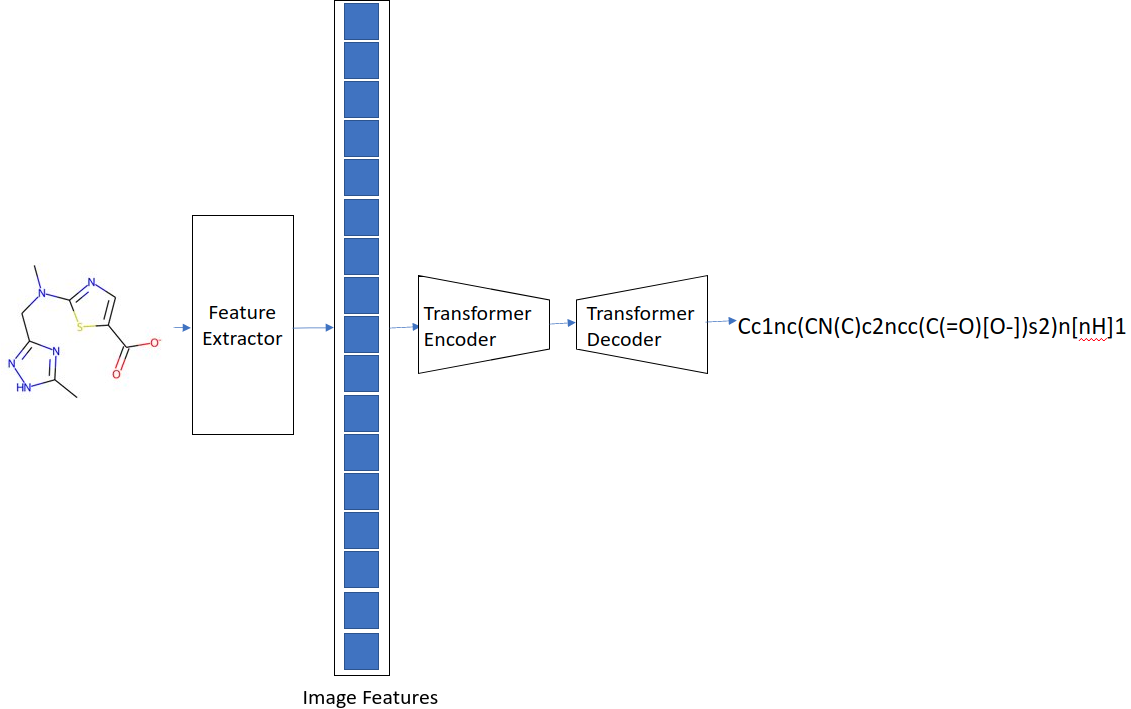
\includegraphics[height=7cm]{image/captioning-task.png}
\caption{Our image captioning system relies on a RESNET-101 based system to extract features from each molecule image followed by a transformer based encoder and decoder to produce candidate SMILES strings.}
\label{fig:system description}
\end{figure}


In summary, the main contributions of this paper are as follows:
\begin{enumerate}
    \item We introduce the IMG2SMI molecule prediction model. Using a RESNET-101 backbone and a transformer based encoder-decoder stack it produces 
    \item We introduce a novel dataset named IMG2SMI. The dataset features 80 million p
    \item We provide a through study of methods of processing SMILES strings for image captioning.
\end{enumerate}


\heng{1. define the task}
\heng{2. why the task is important: for human users to disambiguate; for downstream NLP components such as IE and QA to use}
\heng{3. limitation of previous work... did not use embedding representation etc.}
\heng{4. our novelty: we propose a 5-way translation: 2-D structure, 3-D structure, SMILES, natural language description. A novel multi-modal representation. }

\section{Related Work}
\subsection{Molecule Representation}
OSRA does not work well with large molecules or with variants in design nor can it be tuned to a task
Chemgrapher \cite{Oldenhof2020ChemGrapherOG} improves on OSRA producing a python based 
Thousands of scientific publications describe new chemical compounds and investigate their
properties. However, the structure of these chemical compounds are usually described in the
publication only as an image. This means that today a rich source of data, which would be
extremely valuable to develop novel machine learning approaches or simply query documents
more accurately, is largely under-exploited. It is therefore important to convert images of
chemical structures into these formats. A few tools for recognizing graph structures from
chemical compound images are available, such as OSRA [8] and others like ChemReader [18],
Kekule [17], CLiDE Pro [25], and the work of M. Sadawi et al.. However, we observe that,
using these tools, bond multiplicity and stereochemical information are sometimes lost. Those
tools are mainly expert systems using different techniques, such as image processing, optical
character recognition, hand-coded rules, or sophisticated algorithms. Modifying or further
improving these tools requires a lot of effort. A tool based on machine learning, which learns
directly from training data, would be most valuable. Such a tool could potentially become
more accurate than existing methods and its performance could be improved by increasing
the size and the diversity of the data sets, instead of having to modify its code.
Therefore, we propose a new data-driven machine learning based tool that can learn from
only image data to recognize the chemical structure graph given an image of a chemical
structure. The core of the tool is a deep learning model. In the work of Staker et al., another
deep learning model was also proposed. However, there the output is only a text-sequence
representing the graph. In our approach, we focus on directly predicting the graph structure
(i.e., identifying all the nodes and the edges and their labels). The positions of these nodes
and edges in the resulting graph would correspond with the positions in the original image
of the chemical structure. The resulting graph can be later translated to any format (e.g.,
SMILES).

The molecular representation refers to the digital encoding used
for each molecule that serves as input for training the deep learning model. A representation scheme must capture essential structural information about each molecule. Creating an appropriate
representation from a molecular structure is called featurization.
Two important properties that are desirable (but not required)
for representations are uniqueness and invertibility. Uniqueness
2
means that each molecular structure is associated with a single representation. Invertibility means that each representation
is associated with a single molecule (a one-to-one mapping).
Most representations used for molecular generation are invertible, but many are non-unique. There are many reasons for nonuniqueness, including the representation not being invariant to
the underlying physical symmetries of rotation, translation, and
permutation of atomic indexes.
There are several ways to represent graphs for machine learning. The most popular way is the SMILES string representation. 47
3
SMILES strings are a non-unique representation which encode
the molecular graph into a sequence of ASCII characters using
a depth-first graph traversal. SMILES are typically first converted
into a one-hot based representation. Generative models then produce a categorical distribution for each element, often with a softmax function, which is sampled. Since standard multinomial sampling procedures are non-differentiable, sampling can be avoided
during training or a Gumbel-softmax can be used
\subsection{Chem AI}
Most small molecules are easily represented as 2D images (with
some notable exceptions like cubane). Inspired by the success
of Google’s Inception-ResNet deep convolutional neural network
(CNN) architecture for image recognition, Goh et al. developed
“Chemception”, a deep CNN which predicts molecular properties
using custom-generated images of the molecular graph. 61 The
Chemception framework takes a SMILES string in and produces
an 80x80 greyscale image which is actually an array of integers,
where empty space is ‘0’, bonds are ‘2’ and atoms are represented
by their atomic number. 61 Bjerrum et al. extend this idea, producing “images” with five color channels which encode a variety
of molecular features, some which have been compressed to few
dimensions using PCA. 52
When scientists design new molecules for a certain application, they have to synthesize them to check experimentally that they possess the right properties. If they don't, the scientists design new molecules (that can be analogs of the previously synthesized molecules, for example), and iterate until they obtain molecules that satisfy their requirements (properties, performance, price, toxicity, environmental impact, etc.). This iterative process takes a lot of time and money.

Being able to accurately predict the properties of hypothetical molecules would allow researchers to synthesize only the most promising ones and to avoid synthesizing and testing many molecules that don't possess the desired properties. Methods of prediction of molecule properties have been used for a long time, often under the name of Quantitative Structure-Activity Relationships (QSAR) or Quantitative Structure-Property Relationships (QSPR). These methods are usually based on physical laws or empirical relationships relating the structure of molecules (often indirectly, via a set of chosen descriptors) to their properties.

The prediction of molecular properties can also be done using machine learning algorithms. These algorithms have been used to predict properties such as bioactivity, toxicity, solubility, melting points, atomization energies, HOMO/LUMO molecular orbital energies and many other kinds of properties. They are neither based on physical laws nor on manually crafted empirical relationships: they are entirely data-driven. Basically, these AI algorithms are trained by feeding them many examples of molecules and their associated properties (supervised learning). Different regression or classification algorithms can be used, such as linear regression, Support Vector Machines, Random Forests or Neural Networks.

AI-based algorithms are particularely well-suited to problems for which the physical laws that determine the molecular properties to be predicted are not exactly known, or when empirical relationships would be too complicated to establish, eg. because of strong non-linearities or correlations between parameters. Interestingly, AI can be used in combination with other prediction methods such as physical equations or empirical relationships, in order to obtain predictions that are even more accurate. For example, AI can use the results of predictions made by physical or empirical relationships as input data, a technique called stacking.

Several deep learning algorithms have been used to design new molecules: variational autoencoders, adversarial autoencoders, recurrent neural networks and graph convolutional networks. These algorithms generate molecular structures either as SMILES strings or directly as graphs, a more recent technique. These deep learning algorithms need to be trained on large numbers of molecules, typically millions, to construct a statistical distribution of the molecules. Several datasets containing millions of molecules are freely available, such as the ZINC database, the QM9 dataset of the ChEMBL database and can be used as training datasets. When generating SMILES strings, it is necessary to check the validity of the generated strings in order to eliminate invalid SMILES. In addition, when using this kind of algorithms, one should verify that the generated molecules are effectively different from the molecules of the training dataset and measure the chemical diversity of the generated molecules (how different they are from known molecules).
\subsection{Molecule Extraction}
Chem Grapher\cite{Oldenhof2020ChemGrapherOG} 
\subsection{Image Captioning}


We DETR \cite{Carion2020EndtoEndOD}

\cite{Bajusz2015WhyIT}

1. Formally define task
2. Describe dataset construction and size
3. Describe Metrics and reasing 
%wget https://raw.githubusercontent.com/undeadpixel/reinvent-randomized/master/training_sets/chembl.training.smi
%wget https://raw.githubusercontent.com/undeadpixel/reinvent-randomized/master/training_sets/chembl.validation.smi

%wget https://raw.githubusercontent.com/undeadpixel/reinvent-randomized/master/training_sets/decorator_scaffolds_drd2.training.smi
%wget https://raw.githubusercontent.com/undeadpixel/reinvent-randomized/master/training_sets/decorator_scaffolds_recap.training.smi
%wget https://raw.githubusercontent.com/undeadpixel/reinvent-randomized/master/training_sets/decorator_scaffolds_drd2.validation.smi
%wget https://raw.githubusercontent.com/undeadpixel/reinvent-randomized/master/training_sets/decorator_scaffolds_recap.validation.smi
%wget https://raw.githubusercontent.com/undeadpixel/reinvent-randomized/master/training_sets/gdb13.1M.training.smi
%wget https://raw.githubusercontent.com/undeadpixel/reinvent-randomized/master/training_sets/gdb13.1M.validation.smi
%wget https://raw.githubusercontent.com/alexarnimueller/SMILES_generator/master/data/chembl24_10uM_20-100.csv
%wget https://deepchemdata.s3-us-west-1.amazonaws.com/datasets/pubchem.zip
%wget https://cactus.nci.nih.gov/osra/uspto-validation-updated.zip
%unzip pubchem.zip

%Cc1nc(CN(C)c2ncc(C(=O)[O-])s2)n[nH]1 -> [C][C][=N][C][Branch2_1][Ring1][Ring2][C][N][Branch1_1][C][C][C][=N][C][=C][Branch1_1][Branch1_2][C][Branch1_2][C][=O][O-expl][S][Ring1][Branch2_1][=N][NHexpl][Ring1][S]

A large validation set consisting of 5719 chemical structure images and associated MOL files is available for download. This set was produced from the US Patent Office Complex Work Units and contain one structure per image, ground truth MOL files and a simple Perl script to benchmark the results of your chemical structure recognition software. The benchmark script takes two arguments - first the folder with ground truth files ("molfiles") and second with your generated files - the filenames of individual structures should be identical. It will compare the structures based on standard InChI. This validation set was made possible courtesy of collaboration with Dr. Steve Boyer and Dr. John Kinney.

This file has been updated courtesy of Aniko Valko and Keymodule Ltd., UK. The ground truth molfiles have been corrected and invalid images have been removed.
Download zip archive here.
A subset of 450 images from the Japanese Patent Office Chem-Infty dataset containing only organic molecules can be downloaded here:
images and ground truth.
This subset is distributed by permission from the original Chem-Infty dataset authors Koji Nakagawa, Akio Fujiyoshi, and Masakazu Suzuki. This work is licensed under a Creative Commons Attribution-Noncommercial-No Derivative Works 2.1 Japan License.
\section{Experiment}
\subsection{Dataset Creation}
Data comes from :
\subsection{Implementation}

\section{Experiments}
The most popular similarity measure for comparing chemical structures represented by means of fingerprints is the Tanimoto (or Jaccard) coefficient T. Two structures are usually considered similar if T > 0.85 (for Daylight fingerprints). However, it is a common misunderstanding that a similarity of T > 0.85 reflects similar bioactivities
\subsection{Variation with SMILES Processing method}
 as BPE often splits sequences into tokens which are not
semantically valuable in respect to the SELFIES/SMILES grammar. Further benchmarking on the
entire MoleculeNet suite is needed to validate this idea

BPE is a hybrid between character and word-level representations, which allows for
the handling of large vocabularies in natural language corpora. Motivated by the intuition that rare
and unknown words can often be decomposed into multiple known subwords, BPE finds the best
word segmentation by iteratively and greedily merging frequent pairs of characters [32]. We compare
\begin{table}[b]
\resizebox{\textwidth}{!}{%
\begin{tabular}{|l|l|l|l|l|l|l|l|}
    \hline
        Model Name & Images Captioned & Valid Captions & Levenshtein Distance & BLEU-1 & MACCS Similatiry & Path Similarity & Morgan Similarity \\ \hline
        OSRA(Baseline) & \textbf{86.5} & \textbf{65.2} & \textbf{30.841} & \textbf{0.0533} & \textbf{0.3849} & \textbf{0.2835} & \textbf{0.286} \\ \hline
        SELFI-NET & 61.8 & 61.8 & 53.02 & 0.0289 & 0.1526 & 0.0954 & 0.0451 \\ \hline
        SMI-100-NET & 3.5 & 3.6 & 42.381 & 0.0128 & 0.0073 & 0.0061 & 0.0028 \\ \hline
        SMI-200-NET & 3.5 & 3.5 & 42.379 & 0.0073 & 0.006 & 0.0056 & 0.0022 \\ \hline
        SMI-500-NET & 3.3 & 3.3 & 42.267 & 0.0071 & 0.0068 & 0.0057 & 0.0032 \\ \hline
        SMI-2000-NET & 10.2 & 10.2 & 40.956 & 0.0049 & 0.0515 & 0.027 & 0.0241 \\ \hline
        SMI-20000-NET & 5.4 & 5.4 & 42.187 & 0.0024 & 0.0092 & 0.0074 & 0.0042 \\ \hline
    \end{tabular}}
    \caption{Table 1: Static Encoder. }
\end{table}

\begin{table}[b]
\resizebox{\textwidth}{!}{%
\begin{tabular}{|l|l|l|l|l|l|l|l|l|}
    \hline
        Model Name & Images Captioned & Valid SMILES & Levenshtein Distance & BLEU-1 & MACCS Similatiry & Path Similarity & Morgan Similarity & Image Reconstruction \\ \hline
        OSRA(Baseline)  & 86.5 & 65.2 & \textbf{30.841} & 0.0533 & 0.3849 & \textbf{0.2835} & \textbf{0.286} & \textbf{9.0777} \\ \hline
        SELFI-NET & \textbf{99.4} & \textbf{99.4} & 33.636 & \textbf{0.0549} & \textbf{0.418} & 0.2309 & 0.1328 & 9.5994 \\ \hline
        SMI-100-NET &  2.9 & 2.9 & 38.229 & 0.024 & 0.1551 & 0.0773 & 0.073 & 9.5184 \\ \hline
        SMI-200-NET & 21.5 & 21.5 & 39.544 & 0.0148 & 0.1015 & 0.0473 & 0.0455 & 9.4374 \\ \hline
        SMI-NET & 8.5 & 8.5 & 41.423 & 0.0097 & 0.0385 & 0.0183 & 0.0162 & 9.4737 \\ \hline
        SMI-NET &  20 & 20 & 39.955 & 0.0115 & 0.0787 & 0.0393 & 0.0285 & 9.5625 \\ \hline
        SMI-NET &  18.1 & 18.0 & 41.406 & 0.0042 & 0.0412 & 0.0121 & 0.0139 & 9.4855 \\ \hline
    \end{tabular}}
    \caption{Table 1: Finetune Encoder. }
\end{table}
To explore ...
Self-Referencing Embedded Strings (SELFIES): A 100% robust molecular string representation \cite{Krenn2019SelfReferencingES}
\subsection{Transformer Based IMG2SMI}
Reference File:data/evaluation_labels.smi
Candidate File:outputs/1e5finetune-predictions.txt
There are 5000 examples being evaluated
Percent Captions Generated:0.9952
Percent Valid SMI Generated:0.995
Exact matches for Cannonical SMI strings:144
Levenshtein Distance:23.6692
BLEU-1 using data/tokenizers/tokenizer_vocab_20000.json tokenizer:0.058
MACCS Fingerprinting Tanimoto Similarity:0.7583
RD Path Fingerprinting Tanimoto Similarity:0.5751
Morgan Fingerprint Tanimoto Similarity:0.5079

Reference File:data/evaluation_labels.smi
Candidate File:outputs/3e5finetune-predictions.txt
There are 5000 examples being evaluated
Percent Captions Generated:0.9954
Percent Valid SMI Generated:0.9954
Exact matches for Cannonical SMI strings:343
Levenshtein Distance:21.409
BLEU-1 using data/tokenizers/tokenizer_vocab_20000.json tokenizer:0.0611
MACCS Fingerprinting Tanimoto Similarity:0.9309
RD Path Fingerprinting Tanimoto Similarity:0.8724
Morgan Fingerprint Tanimoto Similarity:0.8362

Reference File:data/evaluation_labels.smi
Candidate File:outputs/5e5base-predictions.txt
There are 5000 examples being evaluated
Percent Captions Generated:0.9958
Percent Valid SMI Generated:0.9958
Exact matches for Cannonical SMI strings:123
Levenshtein Distance:24.6992
BLEU-1 using data/tokenizers/tokenizer_vocab_20000.json tokenizer:0.0584
MACCS Fingerprinting Tanimoto Similarity:0.7674
RD Path Fingerprinting Tanimoto Similarity:0.5724
Morgan Fingerprint Tanimoto Similarity:0.4944


Reference File:data/evaluation_labels.smi
Candidate File:outputs/5e5finetune-predictions.txt
There are 5000 examples being evaluated
Percent Captions Generated:0.9954
Percent Valid SMI Generated:0.9954
Exact matches for Cannonical SMI strings:362
Levenshtein Distance:21.1306
BLEU-1 using data/tokenizers/tokenizer_vocab_20000.json tokenizer:0.0615
MACCS Fingerprinting Tanimoto Similarity:0.9475
RD Path Fingerprinting Tanimoto Similarity:0.902
Morgan Fingerprint Tanimoto Similarity:0.8707

Reference File:data/evaluation_labels.smi
Candidate File:outputs/pyosra-predictions.txt
There are 5000 examples being evaluated
Percent Captions Generated:0.7956
Percent Valid SMI Generated:0.604
Exact matches for Cannonical SMI strings:2
Levenshtein Distance:32.7606
BLEU-1 using data/tokenizers/tokenizer_vocab_20000.json tokenizer:0.0511
MACCS Fingerprinting Tanimoto Similarity:0.36
RD Path Fingerprinting Tanimoto Similarity:0.279
Morgan Fingerprint Tanimoto Similarity:0.2677

\section{Conclusion}
While our system outperforms existing systems the EM ratio is still low. 
-Task specific image encoder
-Usage in molecule property prediction
-Train on larger dataset
-Variation in dataset
\section{Conclusion}

\section*{Broader Impact}

Authors are required to include a statement of the broader impact of their work, including its ethical aspects and future societal consequences. 
Authors should discuss both positive and negative outcomes, if any. For instance, authors should discuss a) 
who may benefit from this research, b) who may be put at disadvantage from this research, c) what are the consequences of failure of the system, and d) whether the task/method leverages
biases in the data. If authors believe this is not applicable to them, authors can simply state this.


\begin{ack}
We would like to thank Hanjun Dai for providing the source implementation of GLN. This work was
partially supported by US National Science Foundation IIS-1718853, the CAREER grant IIS-1553687
and Cancer Prevention and Research Institute of Texas (CPRIT) award (RP190107).
Use unnumbered first level headings for the acknowledgments. All acknowledgments
go at the end of the paper before the list of references. Moreover, you are required to declare 
funding (financial activities supporting the submitted work) and competing interests (related financial activities outside the submitted work). 
\end{ack}

\bibliographystyle{acl_natbib}
\bibliography{bib}
\end{document}